Determine the boundary of the following domains
\begin{teilaufgaben}
\item
$\Omega=\{(x,y)\in\mathbb R^2\,|\, x^2+y^2<25\}$.
\item
$\Omega=\{(x,y)\in\mathbb R^2\,|\, |x|+|y|<1\}$.
\end{teilaufgaben}

\begin{loesung}
\begin{teilaufgaben}
\item
$\Omega$ is a disk with radius $5$, so the boundary is
the circle with radius $5$:
\[
\partial\Omega=\{(x,y)\in\mathbb R^2\,|\, x^2+y^2=25\},
\]
(figure \ref{20000003:fig} left).
\item
Since $|x|=|-x|$ and $|y|=|-y|$ we conclude that $\Omega$ is symmetric
with respect to reflectoins at the $x$- and $y$-axes.
It thus suffices to find the part of the boundary in the first quadrant.
A point $(x,y)$ in the first quadrant is in $\Omega$ precisely
if $x+y<1$ or $y<1-x$.
These are the points below the straight line $y=1-x$.
So $\Omega$ is the interior of the square with corners
$(1,0)$, $(0,1)$, $(-1,0)$ and $(0,-1)$,
and the boundary $\partial\Omega$ is (the boundary of) this square
(figure \ref{20000003:fig} right).
\qedhere
\end{teilaufgaben}
\begin{figure}
\begin{center}
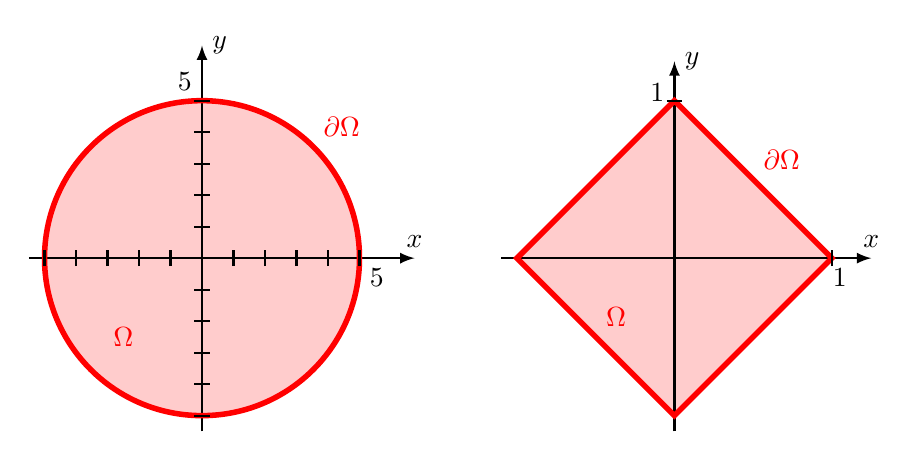
\begin{tikzpicture}[>=latex,thick]
\begin{scope}[xshift=-3cm]
\fill[color=red!20] (0,0) circle[radius=2];
\draw[->] (-2.2,0) -- (2.7,0) coordinate[label={$x$}];
\draw[->] (0,-2.2) -- (0,2.7) coordinate[label={right:$y$}];
\draw[color=red,line width=2.0pt] circle[radius=2];
\node[color=red] at (45:2) [above right] {$\partial\Omega$};
\node[color=red] at (-1,-1) {$\Omega$};
\foreach \x in {1,...,5}{
	\draw ({0.4*\x},-0.1) -- ({0.4*\x},0.1);
	\draw (-0.1,{0.4*\x}) -- (0.1,{0.4*\x});
	\draw ({-0.4*\x},-0.1) -- ({-0.4*\x},0.1);
	\draw (-0.1,{-0.4*\x}) -- (0.1,{-0.4*\x});
}
\node at (2,0) [below right] {$5$};
\node at (0,2) [above left] {$5$};
\end{scope}
\begin{scope}[xshift=3cm]
\fill[color=red!20] (2,0) -- (0,2) -- (-2,0) -- (0,-2) -- cycle;
\draw[->] (-2.2,0) -- (2.5,0) coordinate[label={$x$}];
\draw[->] (0,-2.2) -- (0,2.5) coordinate[label={right:$y$}];
\draw[color=red,line width=2.0pt] (2,0) -- (0,2) -- (-2,0) -- (0,-2) -- cycle;
\node[color=red] at (1,1) [above right] {$\partial\Omega$};
\node[color=red] at (-1,-1) [above right] {$\Omega$};
\draw (2,-0.1) -- (2,0.1);
\draw (-0.1,2) -- (0.1,2);
\node at (2.1,0) [below] {$1$};
\node at (0,2.1) [left] {$1$};
\end{scope}
\end{tikzpicture}
\end{center}
\caption{Domains and boundary for problem \ref{20000003} a) (left)
and b) (right)\label{20000003:fig}}
\end{figure}
\end{loesung}
